
% % This LaTeX was auto-generated from MATLAB code.
% % To make changes, update the MATLAB code and republish this document.
% 
% \documentclass{article}
% \usepackage{graphicx}
% \usepackage{color}
% 
% \sloppy
% \definecolor{lightgray}{gray}{0.5}
% \setlength{\parindent}{0pt}
% 
% \begin{document}

    
    
\section{Test script (castest\_CESneige.m)}\label{par:castest}

\begin{par}
\textbf{Author: Simon Gascoin (CNRS/CESBIO)}
\end{par} \vspace{1em}
\begin{par}
\textbf{June 2015}
\end{par} \vspace{1em}
\begin{par}
This code is a demonstrator of the snow detection algorithm for Sentinel-2 images. It calls the function S2snow (appendix~\ref{par:s2snow}) using subsets of SPOT-4 or Landsat-8 level 2A images.
\end{par} \vspace{1em}
\begin{par}
The input files were generated from L2 images downloaded from Theia Land and pre-processed by three shell scripts:
\end{par} \vspace{1em}
\begin{enumerate}
\setlength{\itemsep}{-1ex}
   \item \texttt{decompresse\_*.sh},        to unzip the files
   \item \texttt{decoupe\_*.sh},        to extract a rectangle AOI from L2A data using       gdal\_translate with projection window defined in the ascii file       \textit{AOI\_test\_CESNeige.csv}
   \item \texttt{projette\_mnt\_*.sh},        to project the SRTM DEM and resample at 30m or 20m       (Landsat8 or Take5) over the same AOI. It uses gdalwarp with the       cubicspline option
\end{enumerate}

\subsection*{Contents}

\begin{itemize}
\setlength{\itemsep}{-1ex}
   \item Configuration
   \item Cloud mask processing parameters
   \item Snow detection parameters
   \item Definition of the input images
   \item Data loading
   \item Snow detection
   \item Figures
\end{itemize}
\begin{par}
Check Matlab version
\end{par} \vspace{1em}
\begin{verbatim}
matlabversion=version;
assert(str2double(matlabversion(end-5:end-2))>=2014,...
    'Needs Matlab version 2014 and later')
\end{verbatim}


\subsection*{Configuration}

\begin{par}
This demo can run for only one image (option 1) or process several images series from different sites and sensors (option 2)
\end{par} \vspace{1em}
\begin{verbatim}
demotype=1;
\end{verbatim}
\begin{par}
If this flag QL is true the code will output three figures for each image
\end{par} \vspace{1em}
\begin{enumerate}
\setlength{\itemsep}{-1ex}
   \item a bar graph showing the snow fraction per elevation band,
   \item a bar graph showing the snow, cloud and elevation area in m2,
   \item a false color composite image overlaid by snow and cloud masks.
\end{enumerate}
\begin{verbatim}
QL=true;
\end{verbatim}
\begin{par}
Define the output path for the figures
\end{par} \vspace{1em}
\begin{verbatim}
pout='../figures/demo_CESneige';
\end{verbatim}
\begin{par}
Define a label to add to the figure file names
\end{par} \vspace{1em}
\begin{verbatim}
label='ndsipass2_015_cloudpass1_bicubic';
\end{verbatim}


\subsection*{Cloud mask processing parameters}

\begin{par}
Resampling factor to determine the "dark clouds" in the initial cloud mask. Here rf=8 corresponds to a target resolution of 240m for Landsat.
\end{par} \vspace{1em}
\begin{verbatim}
rf=8;
\end{verbatim}
\begin{par}
Dark cloud threshold (reflectance unit: per mil). The clouds pixels with a (coarse) reflectance lower than rRed\_darkcloud are selected to pass the snow test
\end{par} \vspace{1em}
\begin{verbatim}
rRed_darkcloud=500;
\end{verbatim}
\begin{par}
Back to cloud threshold. Pixels which are not detected as snow then they go back to the cloud mask only if their reflectance at full resolution is greater than rRed\_backtocloud. Here we use full resolution reflectances because resampled cloud pixels reflectance drops rapidly along the cloud edges due to the mixing with the land reflectance.
\end{par} \vspace{1em}
\begin{verbatim}
rRed_backtocloud=100;
\end{verbatim}


\subsection*{Snow detection parameters}

\begin{par}
Elevation band height in m.
\end{par} \vspace{1em}
\begin{verbatim}
dz=100;
\end{verbatim}
\begin{par}
NDSI threshold for pass 1
\end{par} \vspace{1em}
\begin{verbatim}
ndsi_pass1=0.4;
\end{verbatim}
\begin{par}
Threshold in the red reflectance for pass 1
\end{par} \vspace{1em}
\begin{verbatim}
rRed_pass1=200;
\end{verbatim}
\begin{par}
NDSI threshold for pass 2
\end{par} \vspace{1em}
\begin{verbatim}
ndsi_pass2=0.15; % Note: Zhu's fmask algorithm uses 0.15
\end{verbatim}
\begin{par}
Threshold in the red reflectance for pass 2
\end{par} \vspace{1em}
\begin{verbatim}
rRed_pass2=120;
\end{verbatim}
\begin{par}
Minimum snow fraction from which to compute the snowline elevation (zs)
\end{par} \vspace{1em}
\begin{verbatim}
fsnow_lim=0.1;
\end{verbatim}
\begin{par}
Snow fraction limit to go to pass 2. The total snow fraction after pass 1 is computed to decide whether or not proceed to pass 2. If the snow fraction is below fsnow\_total\_lim then pass 2 is skipped because the number of snow pixels is not sufficient to properly determine the snow line elevation. Here we use 1000 pixels.
\end{par} \vspace{1em}
\begin{verbatim}
fsnow_total_lim=0.001; % Warning! it depends on the image size
\end{verbatim}


\subsection*{Definition of the input images}

\begin{verbatim}
switch demotype
    case 1
\end{verbatim}
\begin{par}
use only 1 image
\end{par} \vspace{1em}
\begin{verbatim}
        satlist={'Take5'};
        sitelist{1}={'Maroc'};
        datelist{1}{1}={'20130327'}; % format yyyymmdd
\end{verbatim}
\begin{verbatim}
    case 2
\end{verbatim}
\begin{par}
process a batch of 2 x Landsat8 and 4 x Take5 images series
\end{par} \vspace{1em}
\begin{verbatim}
        [satlist,sitelist,datelist]=load_demo_input('all');
\end{verbatim}
\begin{verbatim}
    otherwise
        error('demotype should be 1 or 2')
end
\end{verbatim}


\subsection*{Data loading}

\begin{par}
Begin the sensor loop
\end{par} \vspace{1em}
\begin{verbatim}
nsat=length(satlist);
for isat=1:nsat
\end{verbatim}
\begin{verbatim}
    sat=satlist{isat};

    nsite=length(sitelist{isat});
\end{verbatim}
\begin{par}
Get the sensor band numbers and no-data value
\end{par} \vspace{1em}
\begin{verbatim}
    switch sat
        case 'Take5'
            nGreen=1; % Index of green band
            nMIR=4; % Index of SWIR band (1 to 3 µm) = band 11 (1.6 µm) in S2
            nRed=2; % Index of red band
            nodata=-10000; % no-data value
        case 'Landsat8'
            nGreen=3;
            nMIR=6;
            nRed=4;
            nodata=-10000;
        otherwise
            error('sat should be Take5 or Landsat8')
    end
\end{verbatim}
\begin{par}
Begin the site loop
\end{par} \vspace{1em}
\begin{verbatim}
    for isite=1:nsite;
\end{verbatim}
\begin{verbatim}
        site=sitelist{isat}{isite};
        ndate=length(datelist{isat}{isite});
\end{verbatim}
\begin{par}
read SRTM DEM for this site
\end{par} \vspace{1em}
\begin{verbatim}
        fdem=['../' sat '/AOI_test_CESNeige/SRTM/' site '/' site '.tif'];
        [Zdem,R]=geotiffread(fdem);
\end{verbatim}
\begin{par}
Begin the date loop
\end{par} \vspace{1em}
\begin{verbatim}
        for idate=1:ndate
\end{verbatim}
\begin{verbatim}
            date=datelist{isat}{isite}{idate};
\end{verbatim}
\begin{par}
Read the L2 reflectance data (search the image filename based on the date)
\end{par} \vspace{1em}
\begin{verbatim}
            pL2=['../' sat '/AOI_test_CESNeige/LEVEL2A/' site]; % path
            fL2=dir([pL2 '/*' date '*PENTE*.TIF']); % file list
            assert(~isempty(fL2),'The L2 image is not present in the input directory')
            f=[pL2 '/' fL2.name];
            [ZL2,~]=geotiffread(f);
\end{verbatim}
\begin{par}
The data are converted to double because it enables to work with NaN, but we could probably avoid this to optimize memory use..
\end{par} \vspace{1em}
\begin{verbatim}
            ZL2=double(ZL2);
            ZL2(ZL2==nodata)=NaN;
\end{verbatim}
\begin{par}
Read the cloud mask
\end{par} \vspace{1em}
\begin{verbatim}
            fc=dir([pL2 '/*' date '*NUA.TIF']);
            assert(~isempty(fc),'The cloud mask is not present in the input directory')
            f=[pL2 '/' fc.name];
            [Zc,~]=geotiffread(f);
\end{verbatim}


\subsection*{Snow detection}

\begin{par}
Calls the function S2snow (appendix~\ref{par:s2snow})
\end{par} \vspace{1em}
\begin{verbatim}
            [snowtest,cloudtestfinal,z_center,B1,B2,fsnow,zs,...
                fsnow_z,fcloud_z,N,z_edges]...
                = S2snow(...
                ZL2,Zc,Zdem,nGreen,nRed,nMIR,rf,QL,rRed_darkcloud,...
                ndsi_pass1,ndsi_pass2,rRed_pass1,rRed_pass2,dz,fsnow_lim,...
                fsnow_total_lim,rRed_backtocloud);
\end{verbatim}


\subsection*{Figures}

\begin{verbatim}
            if QL
\end{verbatim}
\begin{par}
Draw a bar plot of the snow fraction per elevation band
\end{par} \vspace{1em}
\begin{verbatim}
                figure(1),clf
                barh(z_center,fsnow_z,1,'facecolor','c');
                hold on
                if ~isempty(zs)
                    hrf=refline(0,zs);
                    set(hrf,'Color','r','LineStyle','--','LineWidth',2)
                end
                xlabel('Fractional area')
                ylabel('Elevation (m)')
                legend('Snow','zs')
                title(sprintf('%s zs=%g',date,zs))
\end{verbatim}

%         \color{lightgray} \begin{verbatim}Warning: MATLAB has disabled some advanced graphics rendering features by
% switching to software OpenGL. For more information, click <a
% href="matlab:opengl('problems')">here</a>. 
% \end{verbatim} \color{black}
    
\includegraphics [width=4in]{include/castest_CESneige_01.eps}
\begin{par}
Draw a bar plot of the snow area and elevation band area
\end{par} \vspace{1em}
\begin{verbatim}
                figure(2),clf
                [Nz,~,~] = histcounts(Zdem(:),z_edges);
                barh(z_center,Nz,1,'facecolor',.8*[1 1 1]);
                hold on
                barh(z_center,(fcloud_z+fsnow_z).*Nz',1,'facecolor',.5*[1 1 1]);
                barh(z_center,fsnow_z.*Nz',1,'facecolor','c');
                if ~isempty(zs)
                    hrf=refline(0,zs);
                    set(hrf,'Color','r','LineStyle','--','LineWidth',2)
                end
                xlabel('Area (m2)')
                ylabel('Elevation (m)')
                legend('DEM','Cloud','Snow','zs')
                title(sprintf('%s zs=%g',date,zs))
\end{verbatim}

\includegraphics [width=4in]{include/castest_CESneige_02.eps}
\begin{par}
Show an RGB composition overlaid with pass 1 and 2 snow cover polygons. The clouds pixels are in black.
\end{par} \vspace{1em}
\begin{verbatim}
                figure(3),clf
                z=ZL2(:,:,[nMIR nRed nGreen]);
                max_b=[300 300 300];
                z2=zeros(size(z),'uint8');
                for b=1:3
                    z2(:,:,b)=~cloudtestfinal.*double(z(:,:,b))/max_b(b)*255;
                end
                imshow(uint8(z2),'Border','tight')
                hold on
                for k = 1:length(B1)
                    boundary = B1{k};
                    %         if length(boundary)>100
                    plot(boundary(:,2), boundary(:,1), 'y', 'LineWidth', 1)
                    %         end
                end
                if ~isempty(zs)
                    for k = 1:length(B2)
                        boundary = B2{k};
                        %         if length(boundary)>100
                        plot(boundary(:,2), boundary(:,1), 'm', 'LineWidth', 1)
                        %         end
                    end
                end
\end{verbatim}

%         \color{lightgray} \begin{verbatim}Warning: Image is too big to fit on screen; displaying at 67% 
% \end{verbatim} \color{black}
    
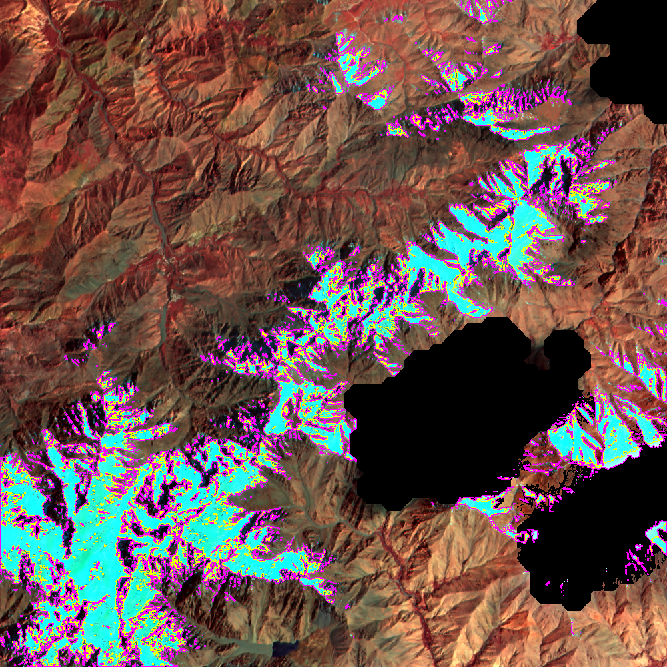
\includegraphics [width=4in]{include/castest_CESneige_03.eps}
\begin{par}
Print figures
\end{par} \vspace{1em}
\begin{verbatim}
                set(1:3,'PaperPositionMode','auto','Visible','off');
                pfig=[pout '/' sat '/' site];
                system(sprintf('mkdir -p %s/zs1',pfig));
                system(sprintf('mkdir -p %s/zs2',pfig));
                system(sprintf('mkdir -p %s/QL',pfig));
                f1=sprintf('%s/zs1/%s_%s_%s_%s.png',pfig,sat,site,date,label);
                f2=sprintf('%s/zs2/%s_%s_%s_%s.png',pfig,sat,site,date,label);
                f3=sprintf('%s/QL/%s_%s_%s_%s.png',pfig,sat,site,date,label);
                print(1,f1,'-dpng')
                print(2,f2,'-dpng')
                print(3,f3,'-dpng')
\end{verbatim}
\begin{verbatim}
            end
\end{verbatim}
\begin{verbatim}
        end
\end{verbatim}
\begin{verbatim}
    end
\end{verbatim}
\begin{verbatim}
end
\end{verbatim}



% \end{document}
    
